\documentclass[UTF8,a4paper,11pt]{ctexart}

\usepackage[margin=2.4cm]{geometry}
\usepackage{graphicx}
\usepackage{booktabs}
\usepackage{array}
\usepackage{float}
\usepackage{hyperref}
\usepackage{xcolor}
\usepackage{enumitem}
\usepackage{longtable}

\hypersetup{
  colorlinks=true,
  linkcolor=blue,
  urlcolor=blue,
  citecolor=blue
}

\setlist[itemize]{leftmargin=2em}
\setlist[enumerate]{leftmargin=2em}
\renewcommand{\arraystretch}{1.18}
\emergencystretch=2em

\title{\textbf{基于 Grounding DINO 的开放词汇目标检测复现与评估}}
\author{
Student Name: 待补充姓名1, 待补充姓名2, 待补充姓名3\\
Student ID: 待补充学号1, 待补充学号2, 待补充学号3
}
\date{}

\begin{document}

\maketitle

\section{Introduction}

开放词汇目标检测（Open-Vocabulary Object Detection, OVOD）旨在使检测模型能够根据任意文本描述定位图像中的目标，而不是只能识别训练集中预定义的固定类别。例如，传统目标检测模型通常只能检测 COCO 中的 80 个类别，而开放词汇检测模型可以通过文本提示词（prompt）检测 ``the person holding an umbrella''、``a laptop on the table'' 等更灵活的语义目标。

本项目选择 Project 4: Open-Vocabulary Object Detection and Visual Grounding，重点复现并评估 Grounding DINO 在开放词汇目标检测任务上的表现。与经典目标检测相比，开放词汇检测的主要挑战包括：模型需要同时理解图像和自然语言文本；检测类别不再固定，prompt 的设计会直接影响预测结果；文本标签与标准数据集类别之间存在映射问题；小目标、遮挡目标和密集目标仍然容易漏检或误检。

本项目的主要目标是构建一个完整的开放词汇检测实验流程，包括模型推理、COCO 子集构建、量化评估、阈值分析、prompt 改进以及失败案例分析。我们基于 HuggingFace Transformers 中的 Grounding DINO 实现推理流程，并在 COCO val2017 的 20 类子集上进行定量评估。

\section{Related works}

开放词汇目标检测通常依赖视觉-语言模型，将图像区域与文本描述对齐。早期的目标检测方法如 Faster R-CNN、YOLO 系列和 DETR 主要针对固定类别进行训练，而开放词汇检测进一步要求模型能泛化到新的文本类别。

CLIP 通过大规模图文对比学习，将图像和文本映射到共享语义空间，为开放词汇识别提供了基础。OWL-ViT 将视觉 Transformer 与文本编码器结合，可以直接使用文本查询进行目标检测。GLIP 将目标检测任务统一为图文 grounding 问题，通过短语与图像区域的对齐提升开放词汇能力。Grounding DINO 进一步结合 DINO 检测器和文本 grounding 机制，在开放词汇检测和 phrase grounding 上取得了较好的效果。

本项目选择 Grounding DINO 作为主要复现对象，原因是其开源实现成熟，HuggingFace 提供了较稳定的模型接口，同时它能够直接接收文本 prompt 并输出检测框、文本标签和置信度，适合作为课程项目中的复现和评估对象。

\section{Method}

\subsection{整体流程}

本项目实现的流程如下：
\begin{enumerate}
  \item 输入图像和文本 prompt；
  \item 使用 Grounding DINO 进行开放词汇检测；
  \item 输出检测框、文本标签和置信度；
  \item 将预测结果可视化；
  \item 将预测结果转换为 COCO detection 格式；
  \item 使用 COCOeval 计算 AP、AP50、AP75 和 AR 等指标；
  \item 对不同 threshold 和 prompt 策略进行对比分析；
  \item 导出 false positive 和 false negative 失败案例。
\end{enumerate}

\subsection{Grounding DINO 推理}

我们没有从头训练模型，而是使用预训练的 Grounding DINO 模型进行 zero-shot 推理。本文所有正式定量实验统一使用 HuggingFace 模型 \texttt{IDEA-Research/grounding-dino-base}。这样可以避免不同模型规模带来的干扰，使实验重点集中在 threshold、prompt 方式和后处理策略对开放词汇检测结果的影响。

\subsection{Prompt 设计}

基础 prompt 使用 COCO 20 类类别名，统一转为英文小写，并用句号分隔。例如：

\begin{verbatim}
a person. a bicycle. a car. a motorcycle. a bus. a truck. ...
\end{verbatim}

在基础方法中，我们将 20 个类别放在同一个 prompt 中一次性推理。这种方式速度较快，但模型有时会输出混合标签，例如 \texttt{traffic light an umbrella}，从而影响类别映射和评估。

为改进这一问题，我们实现了 per-class prompt 策略：每次只查询一个类别，例如 \texttt{a person.}、\texttt{a car.}、\texttt{a traffic light.}，然后将每个类别的检测结果合并。该方法速度明显变慢，但可以避免多类别 prompt 造成的文本标签混乱，并提高 recall。

\subsection{后处理：NMS}

per-class prompt 会产生更多候选框，因此我们进一步加入同类别 NMS（Non-Maximum Suppression）。对于同一类别、同一图像中的预测框，如果 IoU 大于 0.5，则只保留置信度最高的框。最终改进方法为：

\begin{center}
\texttt{per-class prompt + per-label NMS, IoU threshold = 0.5}
\end{center}

\section{Experiments}

\subsection{Datasets}

本项目使用 COCO val2017 作为评估数据来源。为了控制实验规模并贴合开放词汇检测任务，我们从 COCO val2017 中选取 20 个常见类别：

\begin{verbatim}
person, bicycle, car, motorcycle, bus, truck, traffic light,
dog, cat, horse, chair, couch, dining table, bottle, cup,
laptop, book, backpack, umbrella, cell phone
\end{verbatim}

本文主要实验使用 1000 张图片正式实验子集。该子集包含 1000 张图片、20 个类别和 5892 个标注框。数据准备脚本会保留 COCO annotation 格式，方便后续使用 COCOeval 进行标准目标检测评估。

\subsection{Implementation Details}

项目使用 Python 实现，主要依赖 PyTorch、HuggingFace Transformers、Pillow、pycocotools、matplotlib 和 tqdm。主要脚本包括：

\begin{itemize}
  \item \texttt{scripts/infer.py}：执行 Grounding DINO 推理并生成可视化图和 JSON 结果；
  \item \texttt{scripts/prepare\_coco\_subset.py}：构建 COCO 子集；
  \item \texttt{scripts/eval\_coco.py}：将预测结果转为 COCO detection 格式并计算指标；
  \item \texttt{scripts/export\_failure\_cases.py}：导出 false positive 和 false negative 失败案例图。
\end{itemize}

\begin{table}[H]
\centering
\caption{主要实验配置}
\begin{tabular}{ll}
\toprule
配置项 & 设置 \\
\midrule
模型 & \texttt{IDEA-Research/grounding-dino-base} \\
图像数量 & 1000 \\
类别数量 & 20 \\
box threshold & 0.25 \\
text threshold & 0.25 \\
NMS IoU threshold & 0.5 \\
评估工具 & COCOeval \\
\bottomrule
\end{tabular}
\end{table}

\subsection{Metrics}

本项目采用 COCO 目标检测标准指标：

\begin{itemize}
  \item AP：IoU 从 0.50 到 0.95，步长 0.05 的平均精度；
  \item AP50：IoU = 0.50 时的平均精度；
  \item AP75：IoU = 0.75 时的平均精度；
  \item AP\_small / AP\_medium / AP\_large：不同目标尺寸下的 AP；
  \item AR100：每张图最多保留 100 个检测框时的平均召回率。
\end{itemize}

其中 AP 是最主要的综合指标，AP50 更能反映较宽松定位条件下的检测能力，AR100 反映模型是否能够尽可能召回真实目标。

\subsection{Experimental design \& results}

\subsubsection{Threshold 调整}

最初使用默认 threshold：box threshold = 0.40，text threshold = 0.30。在 1000 张 \texttt{grounding-dino-base} 正式实验中，默认 threshold 过于保守，AP 只有 0.0732，AR100 只有 0.0883；降低到 0.25 / 0.25 后，AP 提升到 0.2073，AP50 提升到 0.2975，AR100 提升到 0.3073。继续降低到 0.20 / 0.20 时，有效预测数从 5924 增加到 11272，未匹配预测数从 731 增加到 2188，误检和标签匹配失败变多，AP 下降到 0.1804。因此后续主实验采用 box threshold = 0.25，text threshold = 0.25。

\subsubsection{Multi-class Prompt 与 Per-class Prompt 对比}

1000 张 COCO 子集上的主要结果如表 \ref{tab:main-results} 所示。

\begin{table}[H]
\centering
\caption{1000 张 COCO 子集实验结果}
\label{tab:main-results}
\small
\begin{tabular}{p{5.2cm}rrrrrr}
\toprule
方法 & AP & AP50 & AP75 & AR100 & 有效预测数 & 未匹配数 \\
\midrule
multi-class prompt, 0.40 / 0.30 & 0.0732 & 0.0988 & 0.0820 & 0.0883 & 1263 & 10 \\
multi-class prompt, 0.25 / 0.25 & \textbf{0.2073} & \textbf{0.2975} & \textbf{0.2289} & 0.3073 & 5924 & 731 \\
multi-class prompt, 0.20 / 0.20 & 0.1804 & 0.2780 & 0.1924 & 0.3023 & 11272 & 2188 \\
per-class prompt + NMS & 0.1284 & 0.1592 & 0.1427 & \textbf{0.4478} & 29706 & \textbf{0} \\
per-class + NMS + score cutoff 0.30 & 0.1225 & 0.1500 & 0.1364 & 0.3997 & 20956 & \textbf{0} \\
per-class + NMS + score cutoff 0.35 & 0.1174 & 0.1420 & 0.1308 & 0.3578 & 14872 & \textbf{0} \\
per-class + NMS + score cutoff 0.40 & 0.1122 & 0.1348 & 0.1252 & 0.3239 & 10321 & \textbf{0} \\
\bottomrule
\end{tabular}
\end{table}

从结果可以看出，在 1000 张图片的 \texttt{grounding-dino-base} 实验中，最佳 AP 来自 multi-class prompt, 0.25 / 0.25。per-class prompt + NMS 并没有提高 AP，但它有两个明显效果：第一，未匹配预测数从 731 降到 0，说明逐类别 prompt 消除了混合文本标签导致的类别映射失败；第二，AR100 从 0.3073 提升到 0.4478，说明它能找回更多真实目标。

代价也很明显：per-class prompt + NMS 的有效预测数达到 29706，是 multi-class 0.25 / 0.25 的约 5 倍，false positive 明显增加，因此 precision 和 AP 下降。score cutoff 可以减少预测数量，但同时也会降低 recall，最终 AP 仍低于 multi-class 0.25 / 0.25。

\begin{figure}[H]
\centering
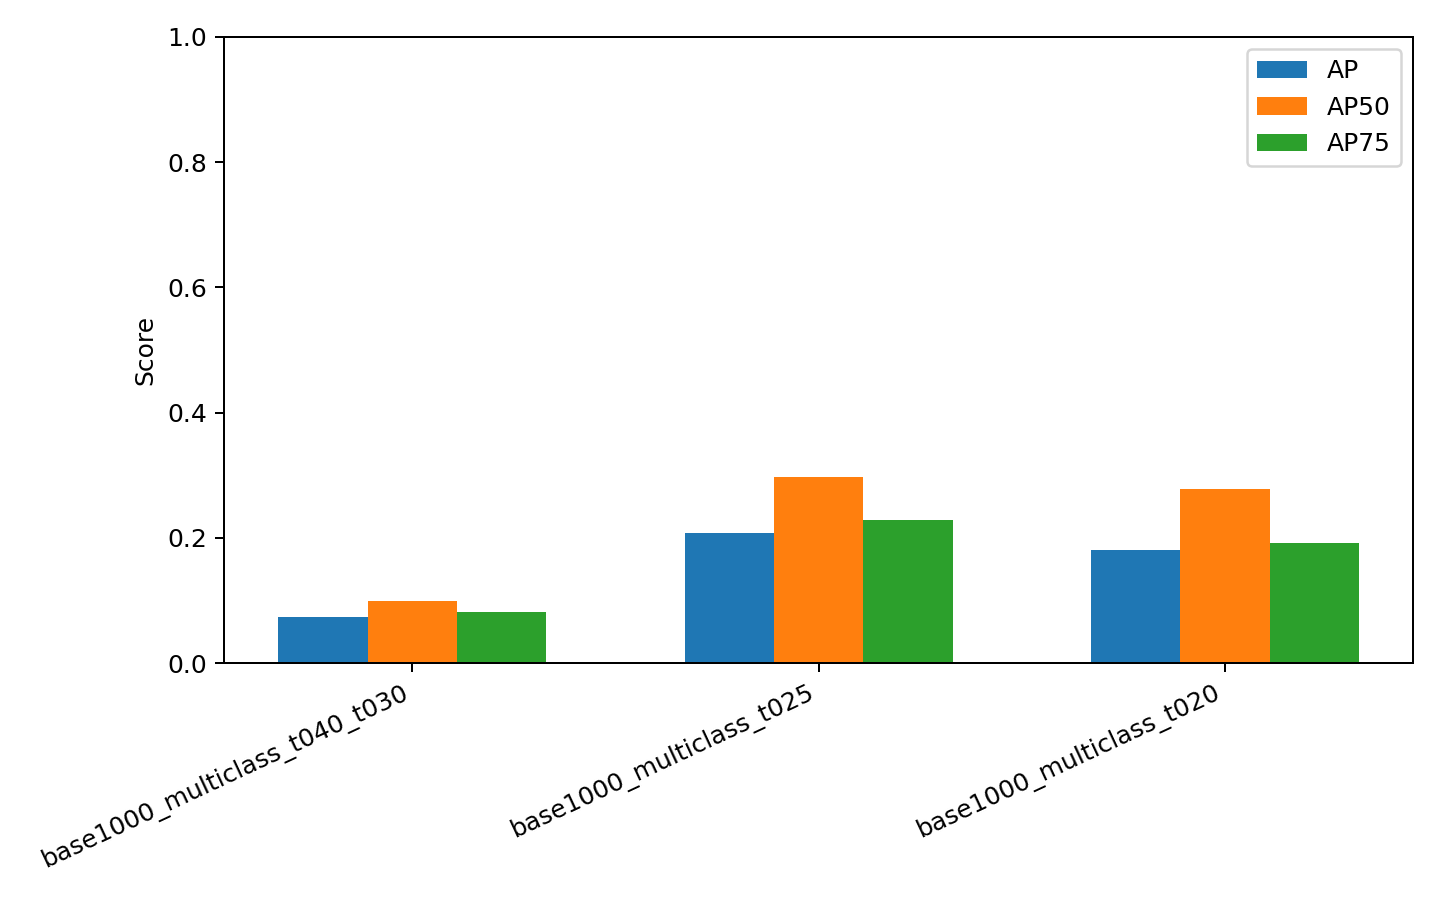
\includegraphics[width=0.92\linewidth]{figures/threshold_comparison_1000_base.png}
\caption{1000 张 COCO 子集 threshold 对比}
\end{figure}

\begin{figure}[H]
\centering
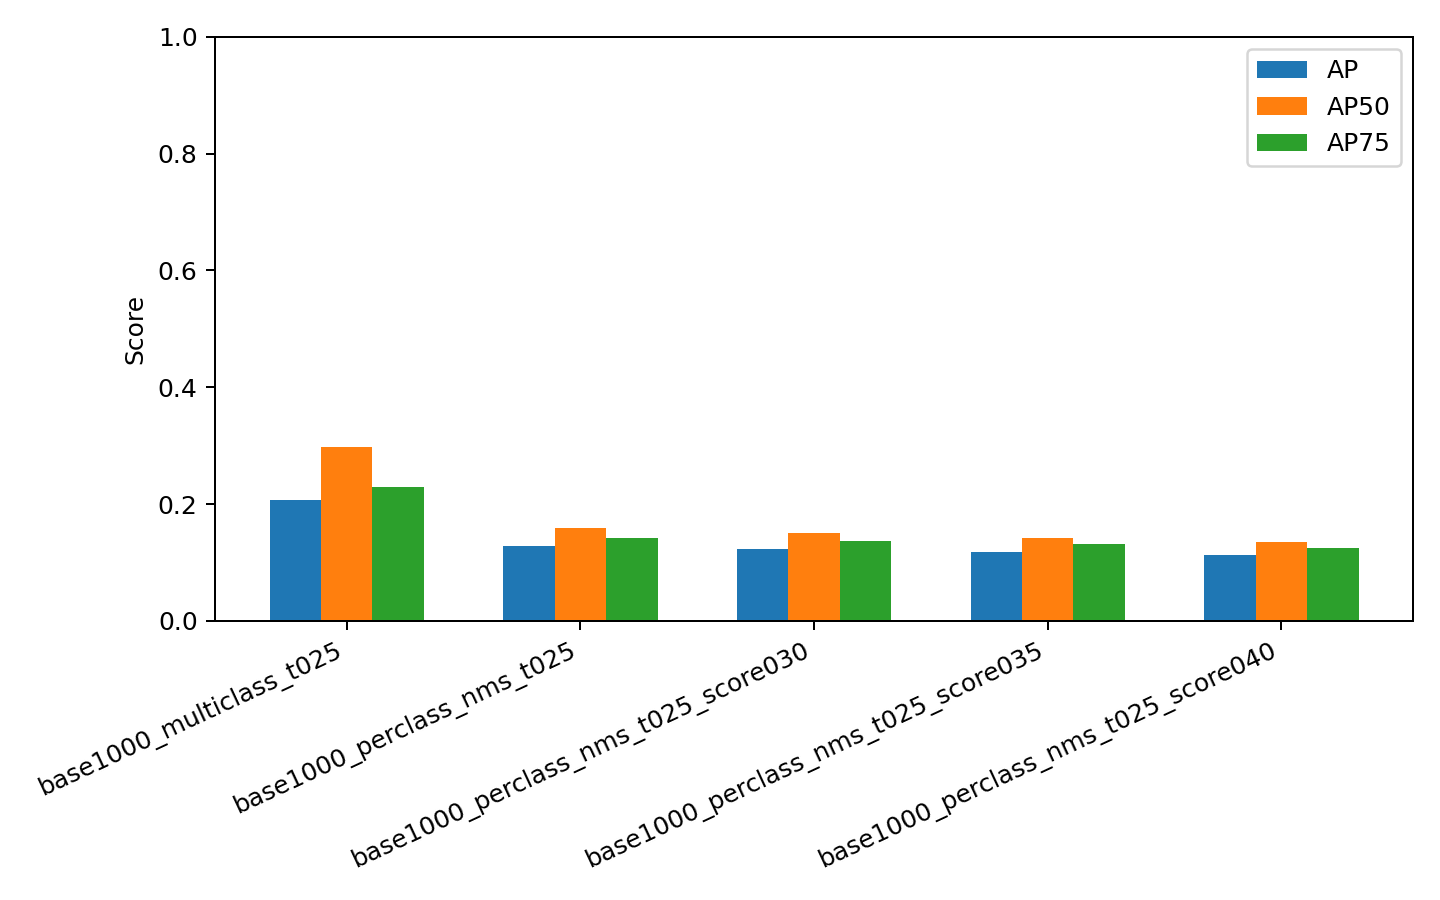
\includegraphics[width=0.92\linewidth]{figures/prompt_comparison_1000_base.png}
\caption{1000 张 COCO 子集 prompt 和 score cutoff 对比}
\end{figure}

\subsubsection{每类 AP 分析}

在最佳配置 multi-class prompt, 0.25 / 0.25 下，表现较好的类别包括 laptop、person、cat、bus、couch 和 cup；表现较差的类别包括 book、dog、truck、bicycle、traffic light 和 cell phone。这说明 Grounding DINO 对大目标、外观清晰的类别更加稳定，而对小目标、遮挡目标和视觉差异较大的类别仍然困难。

\begin{table}[H]
\centering
\caption{最佳配置下 AP 较高的类别}
\label{tab:class-improvement}
\begin{tabular}{lr}
\toprule
类别 & AP \\
\midrule
laptop & 0.6821 \\
person & 0.4329 \\
cat & 0.4196 \\
bus & 0.4046 \\
couch & 0.3252 \\
cup & 0.2362 \\
\bottomrule
\end{tabular}
\end{table}

per-class prompt + NMS 对少数低召回类别有帮助，例如 dog 的 AP 从 0.0347 提升到 0.1910，truck 从 0.0387 提升到 0.1454，bicycle 从 0.0529 提升到 0.0762。但是它也会显著降低一些原本检测较好的类别，例如 laptop 从 0.6821 降到 0.3055，cat 从 0.4196 降到 0.1866，bus 从 0.4046 降到 0.2071。因此，本实验最终将 per-class prompt 视为 recall-oriented 改进，而不是整体 AP 最优方案。

\begin{figure}[H]
\centering
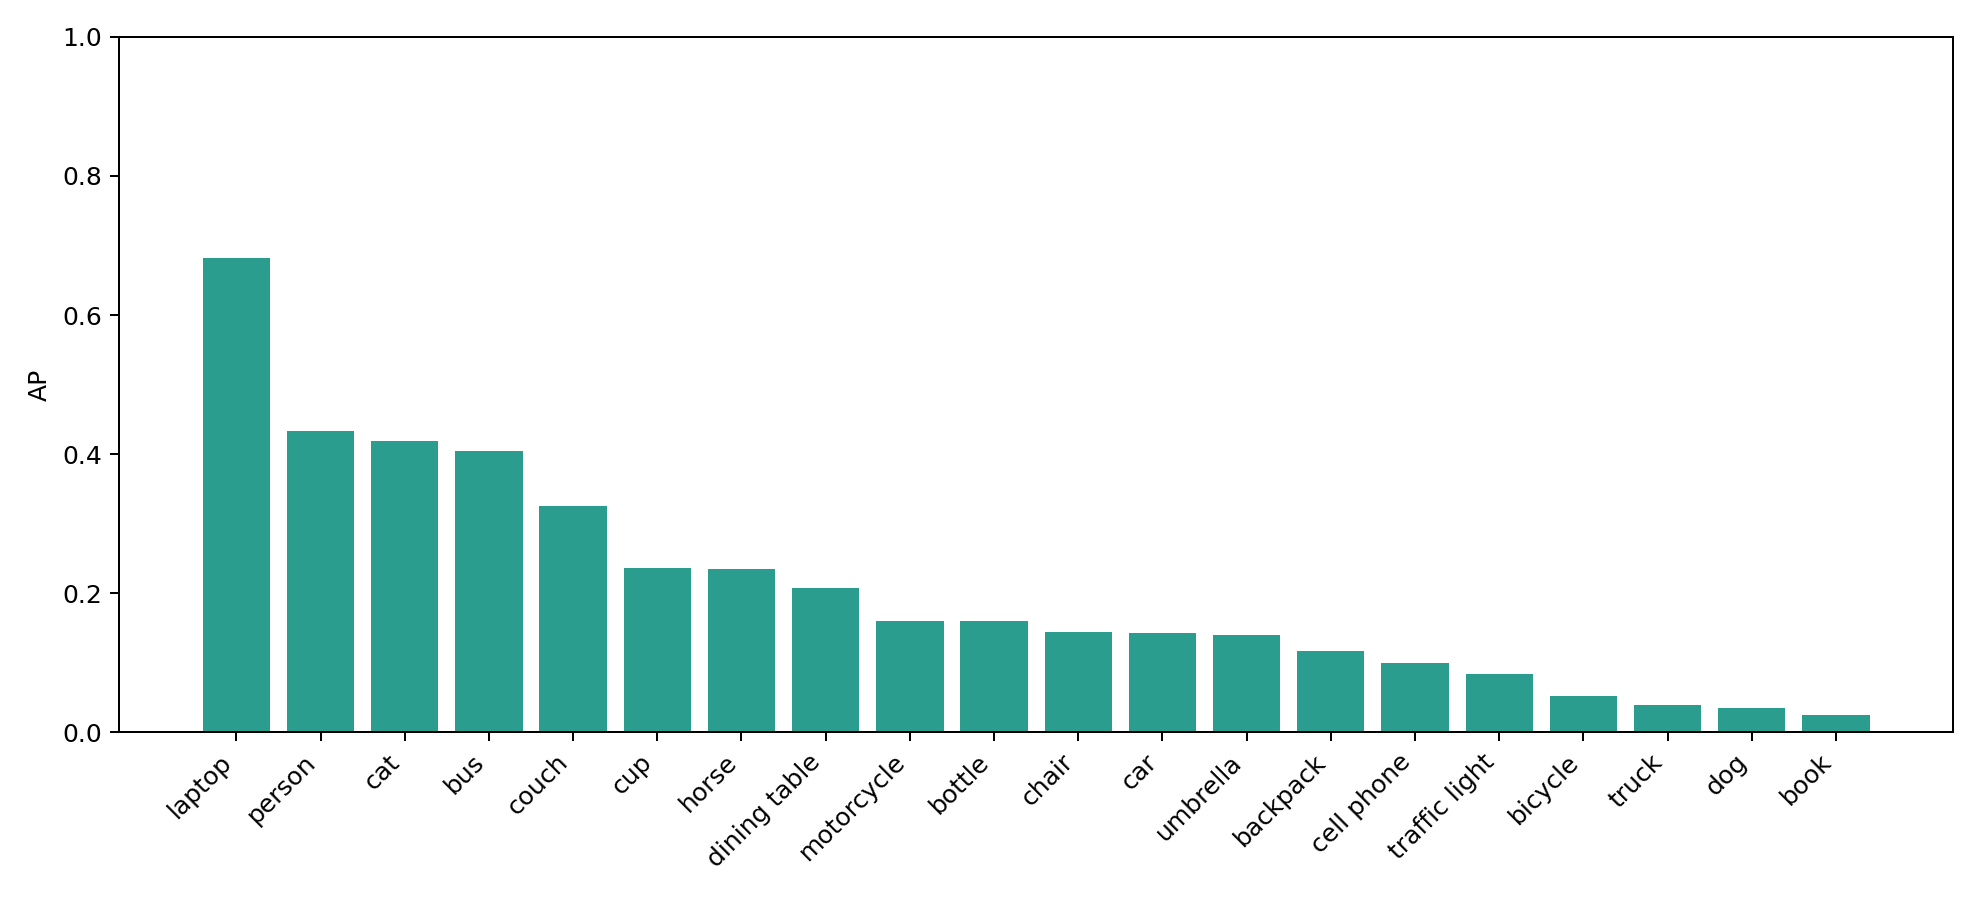
\includegraphics[width=0.92\linewidth]{figures/per_class_ap_1000_base_multiclass_t025.png}
\caption{最佳配置每类 AP}
\end{figure}

\subsubsection{失败案例分析}

我们额外实现了失败案例导出脚本，对预测结果进行 IoU 匹配，并可视化 false positive 和 false negative。图中绿色框表示 ground truth，蓝色框表示 true positive，红色框表示 false positive，橙色框表示 false negative。

典型失败现象包括：小目标漏检，traffic light、book、bottle 等小目标容易被忽略；密集目标误检，多人、多物体场景中容易产生重复框；相似类别混淆，chair 与 couch、bus 与 truck 等类别存在混淆；per-class prompt 提高 recall 后，false positive 数量也增加。

\begin{figure}[H]
\centering
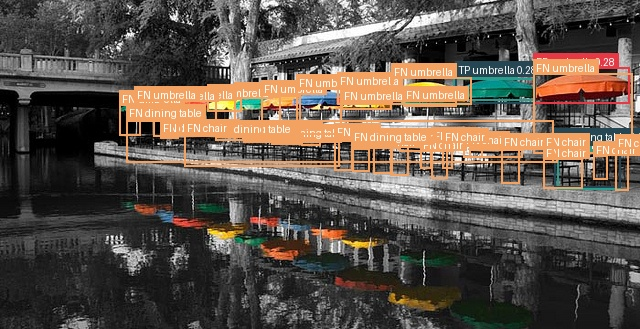
\includegraphics[width=0.82\linewidth]{figures/base1000_multiclass_false_negative_case.jpg}
\caption{Multi-class false negative case}
\end{figure}

\begin{figure}[H]
\centering
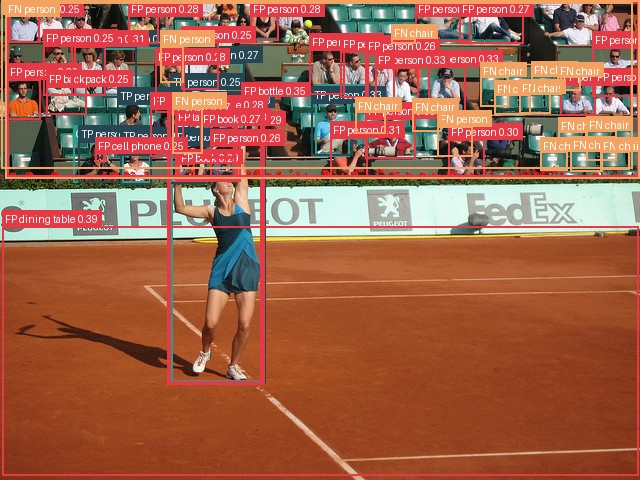
\includegraphics[width=0.82\linewidth]{figures/base1000_perclass_false_positive_case.jpg}
\caption{Per-class false positive case}
\end{figure}

\subsubsection{自采图片 Demo}

本项目还预留了自采图片 demo 流程。用户可以将校园、教室或实验室图片放入自采图片目录，然后使用 person、chair、laptop、bottle、backpack、book、cell phone、cup 等 prompt 进行开放词汇检测。目前仓库中尚未包含真实自采图片，因此本报告暂不展示自采图定量结果。后续补充真实场景图片后，可以作为 presentation 中的 qualitative demo。

\section{Conclusion}

本项目复现了基于 Grounding DINO 的开放词汇目标检测流程，并在 COCO val2017 的 1000 张、20 类子集上完成了定量评估和结果分析。实验表明，threshold 对开放词汇检测性能影响明显，过高阈值会导致严重漏检；将 box threshold 和 text threshold 设为 0.25 后，AP 从 0.0732 提升到 0.2073，AR100 从 0.0883 提升到 0.3073。

进一步地，我们实现了 per-class prompt + NMS 的改进方法。该方法通过逐类别查询减少文本标签混乱问题，将未匹配预测数从 731 降至 0，并将 AR100 从 0.3073 提升到 0.4478。但它同时产生大量候选框，使有效预测数增加到 29706，false positive 增多，AP 下降到 0.1284。因此，本实验最终选择 multi-class prompt, 0.25 / 0.25 作为 AP 最优配置，而将 per-class prompt + NMS 作为提高 recall 和减少标签混乱的补充方案。

未来可以继续探索更好的 prompt 模板、类别自适应阈值、跨类别 NMS、按类别单独调节 score cutoff，以及 YOLO-World 或 GLIP 等其他开放词汇检测模型来进一步提升性能。

\section*{Reference}
\addcontentsline{toc}{section}{Reference}

\begin{enumerate}[label={[\arabic*]}]
  \item S. Liu, Z. Zeng, T. Ren, F. Li, H. Zhang, J. Yang, et al. Grounding DINO: Marrying DINO with Grounded Pre-Training for Open-Set Object Detection. arXiv:2303.05499, 2023.
  \item A. Radford, J. W. Kim, C. Hallacy, A. Ramesh, G. Goh, S. Agarwal, et al. Learning Transferable Visual Models From Natural Language Supervision. ICML, 2021.
  \item M. Minderer, A. Gritsenko, A. Stone, M. Neumann, D. Weissenborn, A. Dosovitskiy, et al. Simple Open-Vocabulary Object Detection with Vision Transformers. ECCV, 2022.
  \item L. H. Li, P. Zhang, H. Zhang, J. Yang, C. Li, Y. Zhong, et al. Grounded Language-Image Pre-training. CVPR, 2022.
  \item T.-Y. Lin, M. Maire, S. Belongie, J. Hays, P. Perona, D. Ramanan, P. Dollár, and C. L. Zitnick. Microsoft COCO: Common Objects in Context. ECCV, 2014.
  \item HuggingFace Transformers Documentation. Grounding DINO model documentation. \url{https://huggingface.co/docs/transformers/model_doc/grounding-dino}
\end{enumerate}

\section*{Contributions}
\addcontentsline{toc}{section}{Contributions}

\begin{itemize}
  \item Name1 (SID1, 35\%): 待补充。建议填写：模型推理与 Grounding DINO 复现、单图/批量推理脚本实现。
  \item Name2 (SID2, 35\%): 待补充。建议填写：COCO 子集构建、COCOeval 评估脚本、量化指标统计。
  \item Name3 (SID3, 30\%): 待补充。建议填写：prompt 改进、NMS 后处理、失败案例分析、报告与展示材料整理。
\end{itemize}

\end{document}
